\documentclass[12pt]{article}
\usepackage[a4paper, left=2.0 cm,right=2.0 cm,top=1.5 cm,bottom=2.0 cm]{geometry}

% load packages that would possibily be used
\usepackage[T1]{fontenc}
\usepackage[UTF8, heading = false, scheme = plain]{ctex}
% self-define title, \@ to reference
\title{Introduction to Machine Learning (HW1)}
\usepackage{fancyhdr}
 \pagestyle{fancy} % set header, disable it if you do not want to include it
 \fancypagestyle{plain}%
 \fancyhf{}
 %\lhead{} % left side of header, could put course code or your name etc.
 \chead{\quad\\[0.2cm] Introduction to Machine Learning (HW1)}
 \rhead{} % right side of header, could put your ID etc.
\usepackage{listings} % code
\usepackage{float} % Package for Float
\usepackage{xcolor} % font color
 \definecolor{mygreen}{rgb}{0,0.6,0}
 \definecolor{mygray}{rgb}{0.5,0.5,0.5}
 \definecolor{mymauve}{rgb}{0.58,0,0.82}
 \definecolor{backcolour}{rgb}{0.95,0.95,0.92}
\usepackage{caption}
\usepackage{palatino}
\usepackage[colorlinks, linkcolor = blue]{hyperref}
\usepackage{titlesec}
\usepackage{amsmath}
\usepackage{amsfonts}
\usepackage{bm}
\usepackage{fancyvrb} % show results of programming
 \newcommand{\VerbBar}{|}
 \newcommand{\VERB}{\Verb[commandchars=\\\{\}]}
 \DefineVerbatimEnvironment{Highlighting}{Verbatim}{commandchars=\\\{\}}
\usepackage{framed}
\usepackage{indentfirst}
 \setlength{\parindent}{2em}
\usepackage{algorithm}  %% to write an algorithm
\usepackage{algorithmicx}
\usepackage[noend]{algpseudocode}
\usepackage{graphicx} % pictures
 \graphicspath{{figures/}} % set image path
\usepackage{subfigure}
\usepackage{multirow}
\usepackage{booktabs}
% set font
\usepackage{mathptmx} % set mathfont to Times New Roman
\usepackage{fontspec}
 \setmainfont{Times New Roman} % Main text font set as Times New Roman
 \newcommand{\consolas}{\fontspec{Consolas}}
 \newcommand{\timesnew}{\fontspec{Times New Roman}}
 \newcommand{\simarab}{\fontspec{Courier New}}
% footnote
\renewcommand{\thefootnote}{\Roman {footnote}}

%---------------------------------------CODE SET-----------------------------------------
\lstset{ %
backgroundcolor=\color{backcolour},      % choose the background color
basicstyle=\footnotesize\consolas,  % size of fonts used for the code
columns=fullflexible,
tabsize=4,
breaklines=true,               % automatic line breaking only at whitespace
captionpos=b,                  % sets the caption-position to bottom
commentstyle=\color{mygreen},  % comment style
escapeinside={\%*}{*)},        % if you want to add LaTeX within your code
keywordstyle=\color{blue},     % keyword style
stringstyle=\color{mymauve}\consolas,  % string literal style
frame=single,
rulesepcolor=\color{red!20!green!20!blue!20},
%identifierstyle=\color{red},
language=python
}
%-------------------------------------MAKETITLE SET---------------------------------------
\makeatletter % change default title style
\renewcommand*\maketitle{%
    \begin{center}% centering title
        \bfseries % bold
        {\LARGE \@title \par} % LARGE font size
        \vskip 1em% %%%  margin 1 em
        {\global\let\author\@empty}%
        {\global\let\date\@empty}%
        \thispagestyle{empty} %  no page style
    \end{center}%
  \setcounter{footnote}{3}%
}
\makeatother

%----------------------------------------BEGIN DOC----------------------------------------
\begin{document}
%---------------------------------------COVER PAGE----------------------------------------
\begin{titlepage}
	\newcommand{\HRule}{\rule{\linewidth}{0.8mm}}
	\quad \\[1.5cm]
	
\includegraphics[width=11cm]{thu-whole-logo.pdf}\\[1cm]
	\center 
	\textsc{\Huge Department of Engineering Physics }\\[0.5cm]
	\textsc{\huge Tsinghua University } \\[2.0cm]
	\makeatletter
	\HRule \\[0.4cm]
	{ \huge \bfseries \@title}\\[0.1cm] 
	\HRule \\[3cm]
	\begin{minipage}{1.0\textwidth}
		\begin{flushleft} \large
			\emph{Author:} \quad \quad \, 姓名 \\[0.15cm]
			\emph{Class:} \quad \quad \; \, 班级 \\[0.15cm]
			\emph{Student ID:} \quad Your ID \\[0.15cm]
			\emph{E-mail:} \quad \quad \; \href{xxx@mails.tsinghua.edu.cn}{xxx@mails.tsinghua.edu.cn} \\[0.15cm]
			\emph{Supervisor:} \quad 教师姓名 \\[0.15cm]
			\emph{Course Code:} \, 1111111 \\
		\end{flushleft}
	\end{minipage}\\[3cm]
	\makeatother
	{\large \today}\\[2cm] 
	\vfill 
\end{titlepage}

\title{\bfseries Homework 1}
%\author{} % add your name if you want to show it in Main text
\date{}
\maketitle
\thispagestyle{fancy}
%------------------------------------------INDEX--------------------------------------
\section{\bfseries Exercise Solution}
 \label{sec:qa}
This part provides you with two methods for homework solution. One could simply use \textcolor{blue}{\simarab $\backslash$section} and the result is exactly the same as what this article shows. Another method would be \textcolor{blue}{\simarab Verbatim}. We could start without any content of exercises like,
\begin{Verbatim}[fontfamily = courier,
                 fontsize = \small,
                 frame = single]
    Exercise 1
\end{Verbatim}

Or, we could start with a full description of the exercise.
\begin{Verbatim}[fontfamily = courier,
                 fontsize = \small,
                 frame = single]
    Exercise 1:
    Consider the optimization problem of soft margin support vector machine, derive the dual form
of this optimization problem and write the corresponding Karush–Kuhn–Tucker (KKT) optimality 
conditions.
\end{Verbatim}

One could adjust the margin between these boxes and main text. Note that verbatim could not wrap automatically which should be done by hand.

\section{\bfseries Formula}
 \label{sec:formula}
The formula can be written with $\$ \cdots \$ $ interline or $\$\$ \cdots \$\$ $ for solitary ones. For a auto numbering formula, one should utilize \textcolor{blue}{\simarab $\backslash$begin\{equation\}} $\cdots$ \textcolor{blue}{\simarab $\backslash$end\{equation\}}.

For example, this shows the interline formula $\mathfrak{R}_n(\mathit{g}) = \mathbb{E}_{\mathit{S}_n \sim \mathit{D}^n} \hat{\mathfrak{R}}_{\mathit{S}_n}(\mathit{g})$. And this is an example of individual line formula.
$$
\begin{cases}
\nabla \times \bm{H} = \bm{J} + \dfrac{\partial \bm{D}}{\partial t} \\
\nabla \times \bm{E} = -\dfrac{\partial \bm{B}}{\partial t} \\
\nabla \cdot \bm{B} = 0 \\
\nabla \cdot \bm{D} = \rho \\
\end{cases}
$$

For formula derivation, one could use \textcolor{blue}{\simarab $\backslash$begin\{aligned\}} $\cdots$ \textcolor{blue}{\simarab $\backslash$end\{aligned\}}. For example,
$$
\begin{aligned}
\sum_{i=1}^n \sum_{j=1}^n a_{ij}x_ix_j &= a_{11}x_1^2 + a_{12}x_1x_2 + \cdots + a_{1n}x_1x_n + \cdots + a_{n1}x_nx_1 + a_{n2}x_nx_2 + \cdots + a_{nn}x_n^2 \\
                                       &= \begin{bmatrix} x_1 & x_2 & \cdots & x_n \end{bmatrix} \begin{bmatrix} a_{11} & a_{12} & \cdots & a_{1n} \\ a_{21} & a_{22} & \cdots & a_{2n} \\ \cdots & \cdots & & \cdots \\ a_{n1} & a_{n2} & \cdots & a_{nn} \end{bmatrix} \begin{bmatrix} x_1 \\ x_2 \\ \cdots \\ x_n \end{bmatrix}
\end{aligned}
$$

Here is the example of auto numbering formula.
\begin{equation}
 \label{equ:1}
 i \hbar \dfrac{\partial \psi}{\partial t} = -\dfrac{\hbar^2}{2m} \nabla ^2 \psi + V \psi
\end{equation}

If one wants to cross reference formulas, one could use this way: \textcolor{blue}{\simarab $\backslash$ref\{label\}} which would induce the following result, as is seen in Equ (\ref{equ:1}).

\section{\bfseries Figure and Table}
 \label{sec:fat}
Here I do not want to bother introducing different ways of inserting figures or constructing tables, one should refer to corresponding documentions for further exploration.

As a simple example of table, one could construct it this way:
\begin{table}[htb]
  \centering
  \caption{Table example}
  \label{tab:example}
    \begin{tabular}{cc}
      \toprule[1.5pt]
      {\heiti col 1} & {\heiti col 2}\\
      \midrule[0.5pt]
      A & some value or data displayed\\
      \bottomrule[1.5pt]
    \end{tabular}
\end{table}

Or, other kinds of tables like Tab \ref{tab:other}.
\begin{table}[H]
  \setlength{\abovecaptionskip}{0pt}
  \setlength{\belowcaptionskip}{-0.2cm}
  \caption{Another example of Table}
  \label{tab:other}
  \begin{center}  
    \begin{tabular}{|l|l|l|l| p{2cm}|}  
    \hline  
    Model & \#parameter & accuracy\\ \hline  
    Faster-RNN & 1M & 0.78 \\ \hline  
    GRU & 2M & 0.72 \\
    \hline  
    \end{tabular}  
  \end{center}  
\end{table}

As to figures, we could change its size with \textcolor{blue}{\simarab scale} parameter. The Fig \ref{fig:example} and Fig \ref{fig:subfigure} shows the different ways of showing figures.
\begin{figure}[ht]
\centering
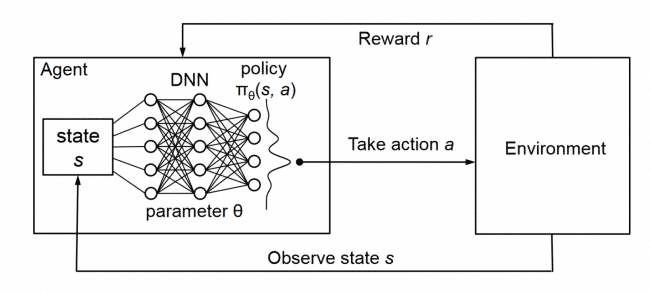
\includegraphics[scale=0.5]{dqn.jpg}
\caption{Figure example}
\label{fig:example}
\end{figure}

\begin{figure}[h]
  \centering%
  \subfigure[Resnet]{
    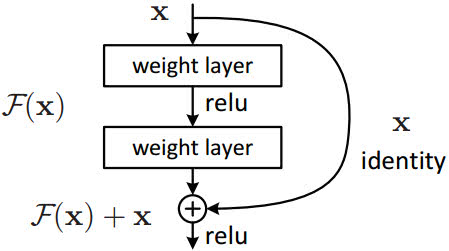
\includegraphics[height=4.5cm]{resnet.jpg}}
  \hspace{4em}%
  \subfigure[MLP]{
    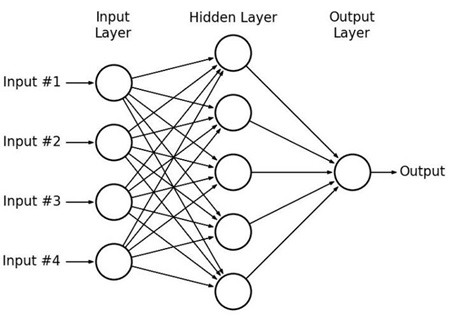
\includegraphics[height=4.5cm]{MLP.jpg}}
  \caption{subfigure example}
  \label{fig:subfigure}
\end{figure}

\section{\bfseries Algorithms and Code Display}
 \label{sec:algcode}
One could write algorithms like the following form:

\begin{algorithm}[H]
\caption{algorithm caption} %name of algorithm
\hspace*{0.02in} {\bf Input:} %input of algorithm
input parameters A, B, C\\
\hspace*{0.02in} {\bf Output:} %output of algorithm
output result
\begin{algorithmic}[1]
\State some description % some general description
\For{condition} % For which need to be corresponded with End For
  \State ...
  \If{condition} % If
    \State ...
  \Else
    \State ...
  \EndIf
\EndFor
\While{condition} % While
  \State ...
\EndWhile
\State \Return result
\end{algorithmic}
\end{algorithm}

Also, if the homework requires one to add codes as an appendix or attach codes in the corresponding exercise, one could utilize \textcolor{blue}{\simarab $\backslash$begin\{lstlisting\}} $\cdots$ \textcolor{blue}{\simarab $\backslash$end\{lstlisting\}}. The following gives a simple example of codes display.
\begin{lstlisting}[language=python, numbers=left]
import numpy as np
from sklearn.tree import DecisionTreeClassifier, export_graphviz
from sklearn.model_selection import train_test_split
from sklearn.datasets import load_breast_cancer
from sklearn.externals.six import StringIO
import graphviz
import pydotplus

# Load data
bc = load_breast_cancer()
X, y = bc.data, bc.target
X_train, X_test, y_train, y_test = train_test_split(X, y, test_size=.3, random_state=1)

# train a classification tree and evaluate it
# set max_depth = 3
dtc = DecisionTreeClassifier(max_depth = 3)
dtc.fit(X_train, y_train)
print("train score:", dtc.score(X_train, y_train))
print("test score:", dtc.score(X_test, y_test))
# visualize the result
dot_data = StringIO()
export_graphviz(dtc, feature_names= bc.feature_names, 
                class_names = bc.target_names,
                out_file = dot_data)
graph = pydotplus.graph_from_dot_data(dot_data.getvalue())
graph.write_pdf("cancer_tree.pdf")
print('Visible tree plot saved as pdf.')
\end{lstlisting}

\section{\bfseries Instruction}
This template is more suitable for math/physics/statistics/computer science. If this template does not meet some of the requirements your homework, you could supplement it yourself.
 
\end{document}